\subsection{SATISFIABILITY RECONFIGURATION}

\begin{frame}{SATISFIABILITY RECONFIGURATION}
    \begin{block}{satisfiability problem}
      The satisfiability problem, also called SAT is to test whether a CNF formula is satisfiable. An example of a CNF formula is $\varphi = (x_1 \vee x_2 \vee \neg x_3) \wedge (x_1 \vee \neg x_2 \vee x_3)$.
    \end{block}

    \begin{block}{Theorem (Cook-Levin)}
      SAT is NP-complete \cite{10.1145/800157.805047}.
    \end{block}

\end{frame}

\begin{frame}{SATISFIABILITY RECONFIGURATION}
    \begin{block}{SAT RECONFIGURATION problems}
       The solutions (satisfying assignments) of a given $n$-variable CNF $\varphi$ induce a subgraph $G(\varphi)$ of the $n$-dimensional hypercube, introducing two decision problems : 
       
       \begin{enumerate}
           \item Connectivity problem : Given a CNF formula $\varphi$, is $G(\varphi)$ connected?
           \item st-Connectivity problem : Given a CNF formula $\varphi$ and two solutions $s_0$ and $s_t$ of $\varphi$, is there a path from $s_0$ to $s_t$ in $G(\varphi)$?
       \end{enumerate}
    \end{block}
\end{frame}

\begin{frame}{SATISFIABILITY RECONFIGURATION}
    \begin{block}{Connectivity $\varphi = (x_1 \vee x_2 \vee \neg x_3) \wedge (x_1 \vee \neg x_2 \vee x_3)$. }
        \begin{columns}
            \begin{column}{0.5\textwidth}
                \begin{figure}
                \centering
                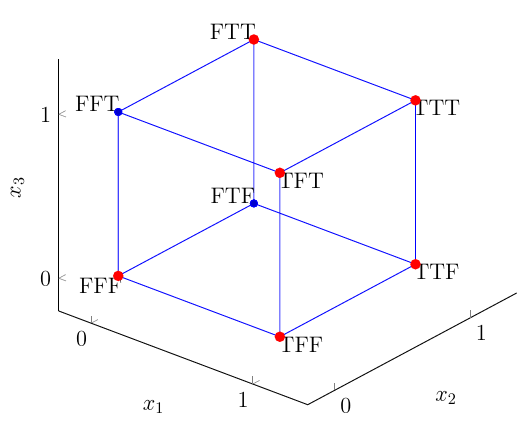
\includegraphics[width=0.9\textwidth]{img/sat_3.png}
                \caption{Reconfiguration graph of $\varphi$.}
                \label{fig:ps}
                \end{figure}
            \end{column}
            \pause
            \begin{column}{0.5\textwidth}
                \begin{figure}
                \centering
                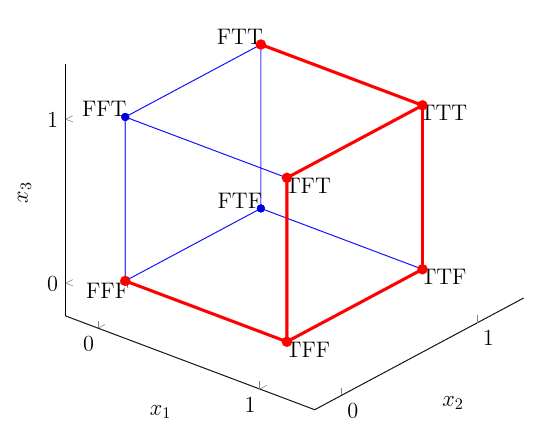
\includegraphics[width=0.9\textwidth]{img/sat_4.png}
                \caption{$G(\varphi)$.\hfill \break}
                \label{fig:circle}
                \end{figure}
            \end{column}
        \end{columns}
    \end{block}
\end{frame}

\begin{frame}{SATISFIABILITY RECONFIGURATION}
    \begin{block}{st-Connectivity $\varphi = (x_1 \vee x_2 \vee \neg x_3) \wedge (x_1 \vee \neg x_2 \vee x_3)$.}
        \begin{columns}
            \begin{column}{0.5\textwidth}
                \begin{figure}
                \centering
                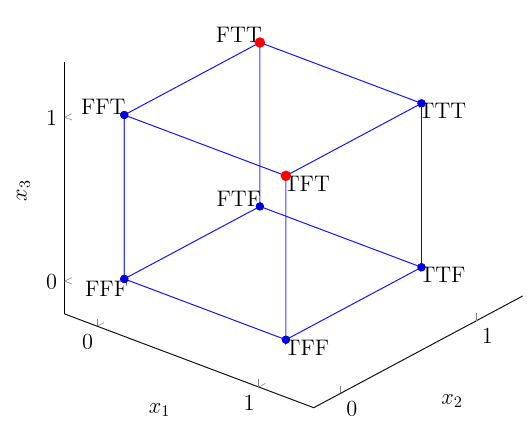
\includegraphics[width=0.9\textwidth]{img/sat_1.png}
                \caption{Reconfiguration graph of $\varphi$ with two satisfying assignments $s_0$ and $s_t$. }
                \label{fig:ps}
                \end{figure}
            \end{column}
            \pause
            \begin{column}{0.5\textwidth}
                \begin{figure}
                \centering
                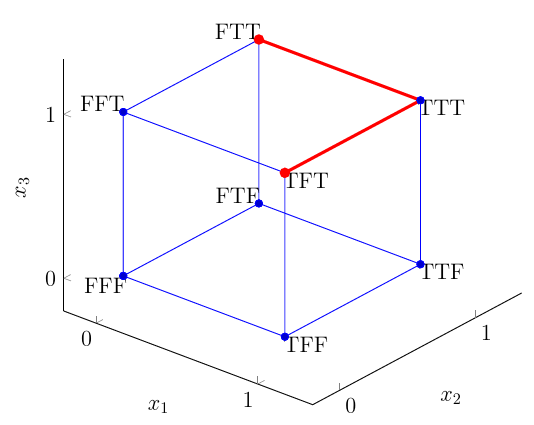
\includegraphics[width=0.9\textwidth]{img/sat_2.png}
                \caption{Reconfiguration sequence transforming $s_0$ to $s_t$. \hfill \break}
                \label{fig:circle}
                \end{figure}
            \end{column}
        \end{columns}
    \end{block}
\end{frame}

\begin{frame}{BOOLEAN SATISFIABILITY RECONFIGURATION}
    \begin{block}{Theorem (Gopalan et al.)}
    The Connectivity problem is PSPACE-complete \cite{gopalan_connectivity_2006}. 
    \end{block}

    \begin{block}{Theorem (Gopalan et al.)}
    The st-Connectivity problem is PSPACE-complete \cite{gopalan_connectivity_2006}. 
    \end{block}

\end{frame}

